\section{組合せ遷移問題と\bm{$k$}彩色遷移問題}\label{chap:background}

\textbf{組合せ遷移問題}
(Combinatorial Reconfiguration Problems;
CoRe~\cite{core:ItoDHPSUU11,core:Nishimura18,core:Heuvel13})
とは,基となる組合せ問題とその2つの実行可能解が与えられたとき,
一方の実行可能解から他方の実行可能解へ,遷移制約を満たしつつ,
実行可能解のみを経由して到達できるかを判定する問題である.
組合せ遷移問題は,基となる組合せ問題の実行可能解が形成する解空間グラフ
を用いて定義される.解空間グラフの頂点は実行可能解を表し,
辺は遷移制約に関する実行可能解の間の隣接関係を表す.
つまり,組合せ問題が実行可能解が存在するかを判定するのに対し,
組合せ遷移問題は,解空間グラフにおいて2つの頂点間の到達可能性を判定
することが目的となる.

計算困難性について,組合せ遷移問題はクラス PSPACE に属する問題である.
基の組合せ問題が NP 完全であるとき,その遷移問題の多くは PSPACE 完全に
なることが知られている.代表的なものとしては,
命題論理の充足可能性判定問題(SAT),
集合被覆問題,
独立点集合,
グラフ点彩色問題を基とする組合せ遷移問題などがある~\cite{%
  core:gcp:BonsmaC09,%
  core:gcp:CerecedaHJ11,%
  core:sat:GopalanKMP09,%
  core:ItoDHPSUU11%
}.

グラフ点彩色問題を基とする組合せ遷移問題は,
\textbf{\bm{$k$}彩色遷移問題}
($k$-coloring Reconfiguration Problems)
ともよばれ盛んに研究されている~\cite{core:gcp:BonsmaC09,core:gcp:CerecedaHJ11}.
$k$彩色遷移問題は,
色数$k$のグラフ点彩色問題と2つの実行可能解が与えられたとき,
一方の実行可能解から他方の実行可能解へ,1回の遷移において色が変化する
頂点はただ1つのみという遷移制約を満たしつつ,実行可能解のみを経由して
到達できるかを判定する問題である~\footnote{%
色数$k$のグラフ点彩色問題とは,与えられた有限無向グラフについて,隣接
する頂点が同色にならないように各頂点を彩色するとき,グラフが$k$色以下
で彩色可能かどうかを判定する問題である.}.
$k$彩色遷移問題では,グラフの形や色数に制限を加えることで多項式時間で
解ける問題が存在するが,一般に$k \ge 4$において PSPACE 完全である.

%%%%%%%%%%%%%%%%%%%%%%%%
\begin{figure}[t]
  \centering
  \scalebox{0.7}{\begin{tabular}{lrrr|r}
  グラフ名 & 頂点数 & 辺数 & 彩色数 & 実行可能解の総数 \\ \hline
  1-FullIns\_3 & 30 & 100 & 4 & 50,693,280 \\ 
  le450\_5a & 450 & 5,714 & 5 & 3,840 \\ 
  le450\_5c & 450 & 9,803 & 5 & 120 \\ 
  le450\_5d & 450 & 9,757 & 5 & 960 \\ 
  myciel3 & 11 & 20 & 4 & 12,480 \\ 
  myciel4 & 23 & 71 & 5 & 2,845,658,400 \\ 
  queen5\_5 & 25 & 160 & 5 & 240 \\  
  queen6\_6 & 36 & 290 & 7 & 100,800 \\ 
  queen7\_7 & 49 & 476 & 7 & 20,160 \\
\end{tabular}}
  \quad
  \scalebox{0.7}{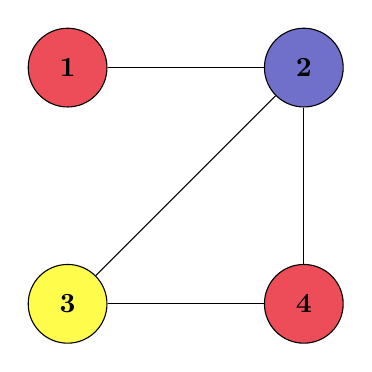
\begin{tikzpicture}[x=1.5cm, y=1.5cm]
  % 設定
  \tikzset{node/.style={circle,draw=black,minimum size=1cm}}
 
  % 色
  \definecolor{red}{RGB}{230,0,18}
  \definecolor{blue}{RGB}{51,51,179}
  \definecolor{yellow}{RGB}{255,251,0}
 
  % 補助線
  % \draw [help lines,blue] (0,0) grid (20,6);
 
  % node %
  \node[node, fill=red!70] at (-1,1) (node1) {\textbf{1}};
  \node[node, fill=blue!70] at (1,1) (node2) {\textbf{2}};
  \node[node, fill=yellow!70] at (-1,-1) (node3) {\textbf{3}};
  \node[node, fill=red!70] at (1,-1) (node4) {\textbf{4}};
 
  \foreach \u / \v in {node1/node2, node2/node3, node2/node4, node3/node4}
  \draw (\u) -- (\v);
\end{tikzpicture}
}
  \caption{色数$k=3$のグラフ点彩色問題の入力例(左)と実行可能解(右)}
  \label{fig:graph}
\end{figure}
%%%%%%%%%%%%%%%%%%%%%%%%

%%%%%%%%%%%%%%%%%%%%%%%%
\begin{figure*}[t]
  \newcommand{\lw}[1]{\smash{\lower-10.ex\hbox{#1}}}
  \begin{tabular}[t]{ccccccc}
    $t=0$ && $t=1$ && $t=2$ && $t=3$ \\
    \scalebox{0.7}{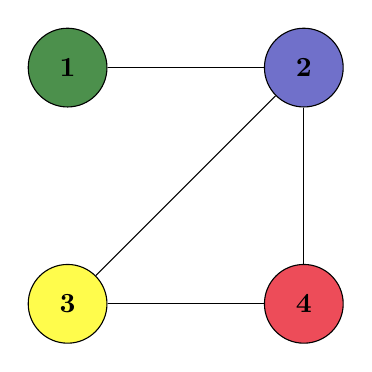
\begin{tikzpicture}[x=1.5cm, y=1.5cm]
  % 設定
  \tikzset{node/.style={circle,draw=black,minimum size=1cm}}
 
  %色
  \definecolor{red}{RGB}{230,0,18}
  \definecolor{blue}{RGB}{51,51,179}
  \definecolor{yellow}{RGB}{255,251,0}
  \definecolor{green}{RGB}{0,96,0}
 
  % 補助線
  % \draw [help lines,blue] (0,0) grid (20,6);
 
  % node %
  \node[node, fill=green!70] at (-1,1) (node1) {\textbf{1}};
  \node[node, fill=blue!70] at (1,1) (node2) {\textbf{2}};
  \node[node, fill=yellow!70] at (-1,-1) (node3) {\textbf{3}};
  \node[node, fill=red!70] at (1,-1) (node4) {\textbf{4}};
 
  \foreach \u / \v in {node1/node2, node2/node3, node2/node4, node3/node4}
  \draw (\u) -- (\v);
\end{tikzpicture}
} &
    \lw{$\Rightarrow$} &
    \scalebox{0.7}{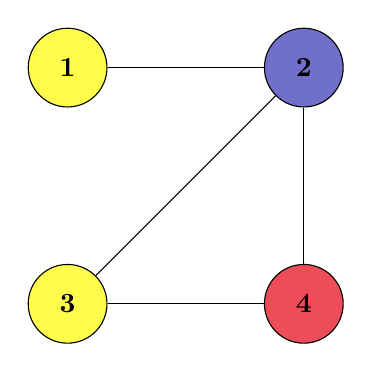
\begin{tikzpicture}[x=1.5cm, y=1.5cm]
  % 設定
  \tikzset{node/.style={circle,draw=black,minimum size=1cm}}
 
  %色
  \definecolor{red}{RGB}{230,0,18}
  \definecolor{blue}{RGB}{51,51,179}
  \definecolor{yellow}{RGB}{255,251,0}
  \definecolor{green}{RGB}{0,96,0}
 
  % 補助線
  % \draw [help lines,blue] (0,0) grid (20,6);
 
  % node %
  \node[node, fill=yellow!70] at (-1,1) (node1) {\textbf{1}};
  \node[node, fill=blue!70] at (1,1) (node2) {\textbf{2}};
  \node[node, fill=yellow!70] at (-1,-1) (node3) {\textbf{3}};
  \node[node, fill=red!70] at (1,-1) (node4) {\textbf{4}};
 
  \foreach \u / \v in {node1/node2, node2/node3, node2/node4, node3/node4}
  \draw (\u) -- (\v);
\end{tikzpicture}
} &
    \lw{$\Rightarrow$} &
    \scalebox{0.7}{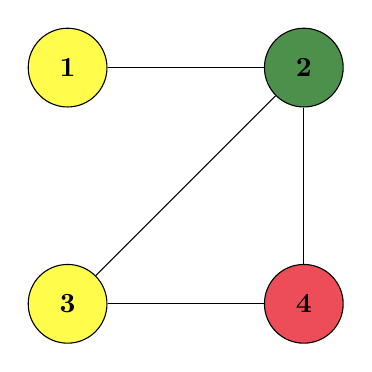
\begin{tikzpicture}[x=1.5cm, y=1.5cm]
  % 設定
  \tikzset{node/.style={circle,draw=black,minimum size=1cm}}
 
  %色
  \definecolor{red}{RGB}{230,0,18}
  \definecolor{blue}{RGB}{51,51,179}
  \definecolor{yellow}{RGB}{255,251,0}
  \definecolor{green}{RGB}{0,96,0}
 
  % 補助線
  % \draw [help lines,blue] (0,0) grid (20,6);
 
  % node %
  \node[node, fill=yellow!70] at (-1,1) (node1) {\textbf{1}};
  \node[node, fill=green!70] at (1,1) (node2) {\textbf{2}};
  \node[node, fill=yellow!70] at (-1,-1) (node3) {\textbf{3}};
  \node[node, fill=red!70] at (1,-1) (node4) {\textbf{4}};
 
  \foreach \u / \v in {node1/node2, node2/node3, node2/node4, node3/node4}
  \draw (\u) -- (\v);
\end{tikzpicture}
} &
    \lw{$\Rightarrow$} &
    \scalebox{0.7}{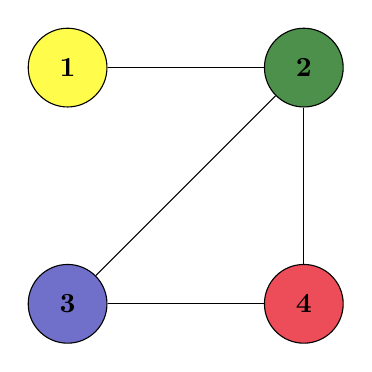
\begin{tikzpicture}[x=1.5cm, y=1.5cm]
  % 設定
  \tikzset{node/.style={circle,draw=black,minimum size=1cm}}
 
  %色
  \definecolor{red}{RGB}{230,0,18}
  \definecolor{blue}{RGB}{51,51,179}
  \definecolor{yellow}{RGB}{255,251,0}
  \definecolor{green}{RGB}{0,96,0}
 
  % 補助線
  % \draw [help lines,blue] (0,0) grid (20,6);
 
  % node %
  \node[node, fill=yellow!70] at (-1,1) (node1) {\textbf{1}};
  \node[node, fill=green!70] at (1,1) (node2) {\textbf{2}};
  \node[node, fill=blue!70] at (-1,-1) (node3) {\textbf{3}};
  \node[node, fill=red!70] at (1,-1) (node4) {\textbf{4}};
 
  \foreach \u / \v in {node1/node2, node2/node3, node2/node4, node3/node4}
  \draw (\u) -- (\v);
\end{tikzpicture}
} \\
    スタート状態 &&&&&& ゴール状態
  \end{tabular}
  \caption{到達可能な$k=4$彩色遷移問題の例}
  \label{fig:gcrp}
\end{figure*}
% start(1,4). start(2,2). start(3,3). start(4,1).
% goal(1,3). goal(2,4). goal(3,2). goal(4,1).
% 1->R, 2->B, 3->Y, 4->G
%%%%%%%%%%%%%%%%%%%%%%%%

図~\ref{fig:graph}に,色数$k=3$のグラフ点彩色問題の例とその実行可能解を示す.
図~\ref{fig:gcrp}は,到達可能な$k=4$彩色遷移問題の例である.
この例は,
スタート状態($t=0$)からゴール状態($t=3$)へ,3ステップの遷移で到達している.
また,各状態$t$はグラフ点彩色問題の制約を満たしており,
1回の遷移においてちょうど1個の頂点の色が変化していることがわかる.

%%% Local Variables:
%%% mode: latex
%%% TeX-master: "paper"
%%% End:
